%-------------------------------------------------------------------------------

% This file is part of Code_Saturne, a general-purpose CFD tool.
%
% Copyright (C) 1998-2016 EDF S.A.
%
% This program is free software; you can redistribute it and/or modify it under
% the terms of the GNU General Public License as published by the Free Software
% Foundation; either version 2 of the License, or (at your option) any later
% version.
%
% This program is distributed in the hope that it will be useful, but WITHOUT
% ANY WARRANTY; without even the implied warranty of MERCHANTABILITY or FITNESS
% FOR A PARTICULAR PURPOSE.  See the GNU General Public License for more
% details.
%
% You should have received a copy of the GNU General Public License along with
% this program; if not, write to the Free Software Foundation, Inc., 51 Franklin
% Street, Fifth Floor, Boston, MA 02110-1301, USA.

%-------------------------------------------------------------------------------

\programme{navstv}\label{ap:navstv}

Consideration is given to solving the non-stationary, pressure-based,
single-phase, three-dimensional Navier-Stokes system of equations for
incompressible or weakly compressible flows based on first-order implicit
Euler or second-order Crank-Nicolson time discretization with collocated
finite volume spatial discretization.


%%%%%%%%%%%%%%%%%%%%%%%%%%%%%%%%%%
%%%%%%%%%%%%%%%%%%%%%%%%%%%%%%%%%%
\section*{Function}
%%%%%%%%%%%%%%%%%%%%%%%%%%%%%%%%%%
%%%%%%%%%%%%%%%%%%%%%%%%%%%%%%%%%%

This subroutine is used to calculate, at a given time step, the velocity
 and pressure variables of the problem following an approach that proceeds
 in two steps based on a decomposition of operators (fractional step method).

The variables are assumed to be known at the instant ${t^n}$ and a
determination of their new values is sought at the
instant\footnote{The pressure is assumed known at instant $t^{n-1+\theta}$
and its new value sought at $t^{n+\theta}$, with $\theta=1$ or $1/2$
depending on the considered time-stepping scheme.} ${t^{n+1}}$.
Therefore, the associated time step is ${\Delta {t^n} ={t^{n+1}- {t^n}}}$.
To begin with, the velocity prediction step is performed by solving the
momentum balance equation with an explicit pressure. This is followed by
the pressure correction (or velocity projection) step allowing to obtain
a null divergence velocity field.

The continuous equations are thus:
\begin{equation}
\left\{
\begin{array}{l}
\displaystyle \der{}{t} \left( \rho \vect{u} \right) + \divv \left( \rho  \vect{u} \otimes \vect{u} \right)
=\divv \left( \tens{\sigma} \right) + \vect{TS} - \tens{K} \cdot \vect{u} + \Gamma \left( \vect{u} - \vect{u}^{in}\right),\\
\der{\rho}{t} + \dive \left( \rho \vect{u} \right) = \Gamma ,
\end{array}\right.
\end{equation}
%
with $\rho$ the density field, $\vect{u}$ the velocity field,
$[\,\vect{TS}-\tens{K}\,\vect{u}\,]$ the other source terms ($\tens{K}$ is a
positive diagonal tensor by definition), $\tens{\sigma}$ the stress tensor,
$\tens{\tau}$ the tensor of viscous stresses,
$\mu$ the dynamic viscosity (molecular and possibly turbulent),
$\kappa$ the volume viscosity (usually null and therefore neglected in
the code and hereafter in this document, apart from the compressible module),
$\tens{D}$ the deformation rate tensor\footnote{Not to be confused,
despite an identical notation $D$, with the diffusive fluxes
$\vect{D}_{\,ij}$ and $\vect{D}_{\,{b}_{ik}}$ described later in this
subroutine.}, $\Gamma$ the mass source term and $\vect{u}^{in}$ is the velocity of the injection.
\begin{equation}
\left\{
\begin{array}{r c l}
\tens{\sigma} & = & \tens{\tau} - P\tens{Id} ,  \\
\tens{\tau} & = & 2 \mu  \tens{D} +  (\kappa  - \frac{2}{3}\mu) tr({\tens{D}})
\tens{Id} , \\
\tens{D} &=& \frac{1}{2}\left( \gradt\vect{u}+ \transpose{\gradt\vect{u}} \right).
\end{array}\right.
\end{equation}

Recalling the definition of the notations employed\footnote{Using the
Einstein summation convention.}:
\begin{equation}\notag
\left\{\begin{array}{r c l}
\left[\gradt{\vect{a}}\right]_{ij} &=& \der{a_i}{x_j},\\
\left[\dive(\tens{\sigma})\right]_i &=& \der{\sigma_{ij}}{x_j},\\
\left[\vect{a}\otimes\vect{b}\right]_{ij} &= &
a_i\,b_j,\\
\end{array}\right.
\end{equation}
and thus:
\begin{equation}\notag
\begin{array}{lll}
\left[\divv(\vect{a}\otimes\vect{b})\right]_i &= &
\der{(a_i\,b_j)}{x_j}
\end{array}
\end{equation}

\begin{remark}
When accounting for variable density, the continuity equation is written:
$$\frac{\partial \rho}{\partial t} + \dive{\,(\rho\,\vect{u})} = \Gamma  $$
This equation is not taken into account in the projection step
(we continue to resolve only $\displaystyle \dive(\,{\rho\,\vect{u}}) = \Gamma$)
whereas the term $\displaystyle \frac{\partial \rho}{\partial t}$ does
appear during the velocity prediction step in the subroutine \fort{predvv}.
If this term plays a significant role, the \CS compressible algorithm
(which solves the full equation) is probably better adapted.
\end{remark}

%%%%%%%%%%%%%%%%%%%%%%%%%%%%%%%%%%
%%%%%%%%%%%%%%%%%%%%%%%%%%%%%%%%%%
\section*{Discretization}
%%%%%%%%%%%%%%%%%%%%%%%%%%%%%%%%%%
%%%%%%%%%%%%%%%%%%%%%%%%%%%%%%%%%%

We define beforehand:
%
\begin{equation}\notag
\displaystyle\alpha_{ij}=\frac{\overline{FJ'}}{\overline{I'J'}} \text{\ defined  at the internal faces only and}
\end{equation}
\begin{equation}\notag
\vect{u}_{K'} = \vect{u}_{K}+(\ggrad{\vect{u}})_K\text{.}\, \vect{KK'}\, \text{\
at first order in space, for ${K = I \,\text{or}\, J}$}
\end{equation}

\begin{figure}[!htbp]
\centering
\subfigure[Internal face.]{
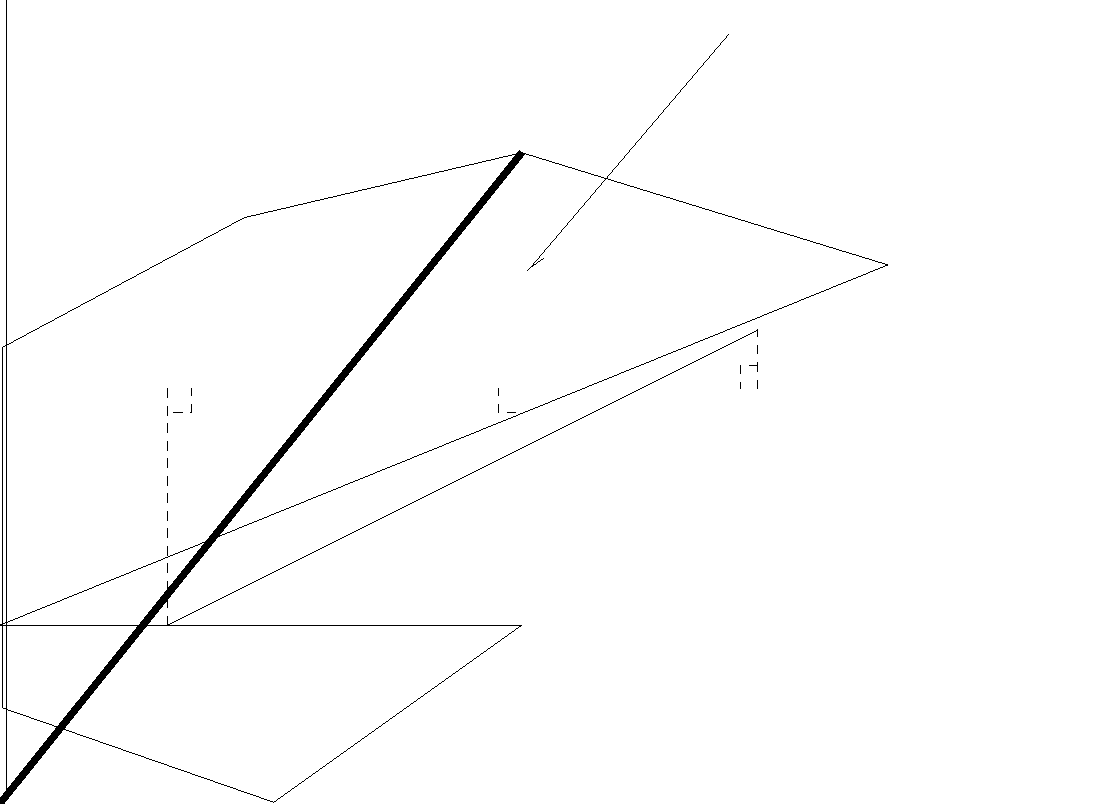
\includegraphics[width=0.4\textwidth]{facette}
}%
\subfigure[Boundary face.]{
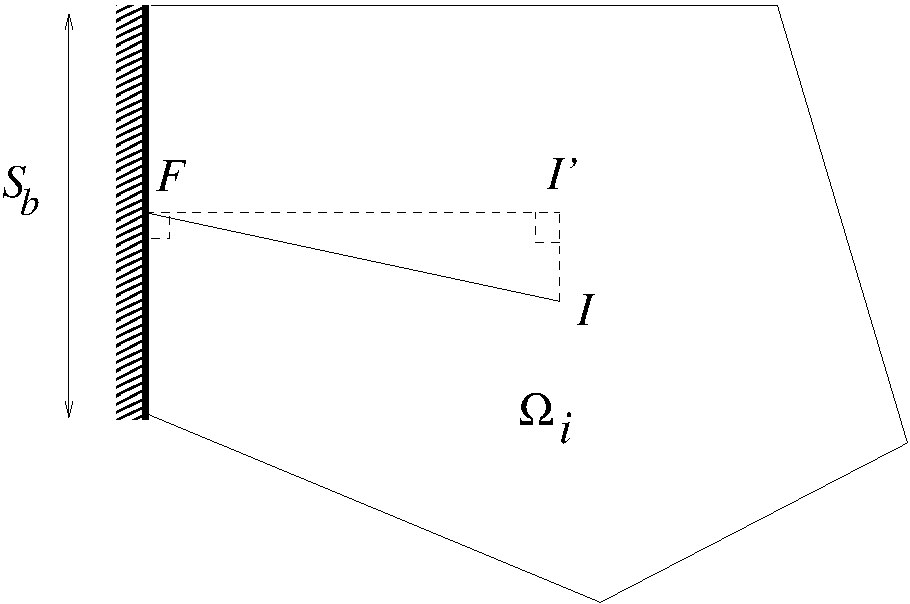
\includegraphics[width=0.4\textwidth]{facebord}
}
\caption{\label{fig:internal_boundary_faces_schetches}Schema of the geometric entities defined for
internal and boundary faces.}
\end{figure}

\subsection*{Fractional step method}
\subsubsection*{Introduction}
One of the methods used to numerically solve the Navier-Stokes equations
consists of decomposing the corresponding operators into a set of simpler
operators (which can then be treated by efficient algorithms) \emph{via}
the division of a single time step into a number of intermediate sub-steps.
In this case, two sub-steps are used: the first takes up the convective,
diffusive and source terms of the momentum equation and constitutes the
velocity prediction step, the second treats the continuity equation and
is designated as the pressure correction or velocity projection step.

\subsubsection*{Velocity prediction step}
The discretization in time is achieved by applying a $\theta$-scheme
at time $n+\theta$ to the resolved variable, following the approach used
for the transport equation of a scalar\footnote{cf. \fort{covofi}}.

The velocity at time $n+1$ not being available until after the projection
step, a predicted velocity at time $n+1$ is used herein to interpolate:
\begin{equation}
\label{eq:navstv:theta_scheme}
\vect{\widetilde{u}}^{n+\theta} = \theta\, {\vect{\widetilde{u}}}^{n+1}+(1-\theta)\, \vect{u}^{n}
\end{equation}
With\footnote{In the $\theta = 1/2$ case, the time step $\Delta t$ is assumed
to be constant in time and uniform in space.} :
\begin{equation}
\left\{
\begin{array}{ll}
\theta = 1   & \text{For a first-order implicit Euler scheme,}\\
\theta = 1/2 & \text{For a second-order Crank-Nicolson scheme.}\\
\end{array}
\right.
\end{equation}

The predicted velocity field ${\vect{\widetilde{u}}^{n+1}}$ is then
obtained by:

\begin{itemize}
\item Partial linearization of the convection operator giving rise to a
decoupling of the velocity components.
\item Explicitation of the pressure.
\item Explicitation or extrapolation of the physical quantities (\emph{i.e}
$\rho,\,\mu,\,Cp\,...$) and the mass flux.
\item Explicitation or extrapolation of the explicit source terms
(for example, the contributions of the transpose gradient, secondary viscosity,
extra diagonal elements of the head losses, injected mass $\Gamma\,\vect{u}^{in}$, ...)
at time $n+\theta_{S}$.
\item The implicit source terms that are linear with respect to the velocity
(implicit user-specified source terms, diagonal of the head losses
$\tens{K_d}\,\underline{u}$, sources of mass $\Gamma\,\vect{u}$, etc...)
are assumed to be evaluated at time $n+\theta$ and are tied to the tensor
$\tens{K}$\footnote{As the velocity components are decoupled, in practice only
the linear terms relative to the resolved component are factorised; the other terms are treated as explicit terms. A more detailed explanation can be found in \fort{predvv}.}.
\end{itemize}

For clarification, unless otherwise specified, the physical properties
$\Phi\,=\,\rho,\,\mu\,...$ and the mass flux $(\rho\vect{u})$ are assumed
to be evaluated respectively at the instants $n+\theta_\Phi$ and
$n+\theta_F$, with $\theta_\Phi$ and $\theta_F$ being dependent on the
specific time-stepping schemes employed for these
quantities\footnote{cf. \fort{introd}}.

After rewriting the non-stationary terms based on the mass conservation relation,
we solve the following system:
\begin{equation}
\displaystyle
\rho\,\left(\dfrac{\vect{\widetilde{u}}^{n+1}-\vect {u}^{n}}{\Delta t}\right) +
\divv \left(\vect{\widetilde{u}}^{n+\theta} \otimes (\rho\vect{u}) \right) =
\divv \left(\tens{\sigma}^{n+\theta}\right) + \vect{TS}^{n+\theta_{S}}-\tens{K}^{n}\,\vect{u}^{n+\theta} +\vect{\widetilde{u}}^{n+\theta}\,\dive{(\rho\vect{u})} ,
\label{eq:navstv:c0_prediction_step}
\end{equation}
with:
\begin{equation}
\displaystyle
\tens{\sigma}^{n+\theta}=\mu\,\,\gradt\vect{\widetilde{u}}^{n+\theta}\underbrace{-P^{n-1+\theta}\tens{Id}+ (\mu \transpose{ \left(\gradt\vect{u})^{n+\theta_{S}}\right)}- \frac{2}{3} ( \mu\, \dive \vect{u})^{n+\theta_{S}}\tens{Id}}_{\text{explicit source terms}}.
\end{equation}

\subsubsection*{\bf Pressure correction step (or projection of velocities)}
The predicted velocity has \emph{a priori} non-zero divergence. The second step
corrects the pressure by imposing the nullity of the stationary constraint for
the velocity computed at time instant ${t^{n+1}}$.
We then solve:
\begin{equation}\label{eq:navstv:c0_correction_step}
\left\{\begin{array}{ r c l}
\displaystyle \dfrac{(\rho\vect{u})^{n+1}-(\rho\vect{\widetilde{u}})^{n+1}}{\Delta t} &=&
-\grad{\delta P^{n+\theta}} ,\\
\displaystyle
\dive(\rho\vect{u})^{n+1} = \Gamma ,\\
\end{array}\right.
\end{equation}

where the pressure increment $\delta P^{n+\theta}$ is defined as:
\begin{equation}
\delta P^{n+\theta}=P^{n+\theta}-P^{n-1+\theta} .
\end{equation}

\begin{remark}
The  $\rho$ and $\mu$ quantities remain constant over the course of both
steps. If there has been any variation in the interval, their values will be modified at the start of the next time step, after the scalars (temperature, mass fraction,...) have been updated.
\end{remark}

\subsection*{Spatial discretization}
Following the classical approach, the time-discretized equations are then integrated over the control volumes ${\Omega_i}$ (or cells).
\subsubsection*{Velocity prediction step}
\paragraph{Second member\\ }
If we do not take account of the $\theta$-scheme convection and diffusion
terms, the explicit volume source terms of the equation \eqref{eq:navstv:c0_prediction_step}
for the system concerning the quantity $(\vect{\widetilde{u}}^{n+1}-\vect {u}^{n})$
	are expressed as:

\begin{equation*}
 -\grad P^{n-1+\theta} + \dive \left[ (\mu \transpose{ \left( \gradt \vect{u}\right) })^{n+\theta_{S}}- \frac{2}{3} ( \mu  \dive \vect{u})^{n+\theta_{S}}\tens{Id} \,\right]+\vect{TS}^{n+\theta_{S}}- \,\tens{K}^{n} \vect{u}^{n}+\vect{u}^{n} \dive{(\rho\vect{u})}.
 \end{equation*}
To integrate these terms over a cell $\vol{\celli}$, we multiply their local value
at the cell centre by the volume of the cell.

\paragraph{Convection  \\}

After decomposition of $\vect{\widetilde{u}}$ based on the relation
\eqref{eq:navstv:theta_scheme}, spatial integration of the convective
parts of the velocity field $\theta\,{\dive\left(\vect{\widetilde{u}}^{n+1}\otimes
(\rho \vect{u})\right)}$ and $(1-\theta)\,{\dive\left(
\vect{u}^{n}\otimes (\rho \vect{u})\right)}$ yields a sum of the numerical
fluxes ${\vect{F}\,_{\,ij}}$ calculated at the faces of the internal cells and ${\vect{F}_{\,b_{ik}}}$ calculated at the boundary faces of the domain $\Omega$.
Taking $Neigh(i)$ as the set of the centres of the neighbouring cells of
${\Omega_i}$ and $\gamma_b(i)$ the set of the centres of the boundary faces of
${\Omega_i}$, we obtain:

\begin{equation*}
\int_{\Omega_i}{\dive\left(\vect{u}\otimes (\rho \vect{u})\right)\, d\Omega} =
\sum_{j\in Neigh(i)}{\vect{F}_{\,ij}((\rho \vect{u}), \vect{u})} \\
+\sum_{k\in {\gamma_b(i)}} {\vect{F}_{\,{b}_{ik}}((\rho \vect{u}),\vect{u})} ,
\end{equation*}
%
with:
\begin{equation}
\vect{F}_{\,ij}((\rho \vect{u}), \vect{u}) = \left[{(\rho \vect{u})_{\,ij}} \text{.}\, \vect{S}_{\,ij}\right]
 \vect{u}_{\,f,ij}.
\end{equation}

\begin{equation}
{\vect{F}_{\,{b}_{ik}}}((\rho \vect{u}),\vect{u}) =  \left[{(\rho \vect{u})_{\,{b}_{ik}}} \text{.}\, \vect{S}_{\,{b}_{ik}}\right]\,{\vect{u}_f}_{\,{b}_{ik}}.
\end{equation}
The value of the flux ${\vect{F}_{\,ij}}$ depends on the numerical scheme
selected. Three different schemes are available in \CS:
%
\begin{enumerate}[ label=\roman{*}/, ref=(\roman{*})]
\item a  first-order upwind scheme:\\
 $\vect{F}_{\,ij}((\rho \vect{u}), \vect{u})=
\vect{F}^{\it{ upwind}}_{\,ij}((\rho \vect{u}),\vect{u})$\\
where:
\begin{equation}
\begin{array}{r c l}
\vect{u}_{\fij}=\vect{u}_{\celli} &\text{ if }&
(\rho \vect{u})_{\fij} \cdot \vect{S}_{\ij} \geqslant 0\\
\vect{u}_{\fij}=\vect{u}_{\cellj} &\text{ if }&
(\rho \vect{u})_{\fij} \cdot \vect{S}_{\ij}  < 0,\\
\end{array}
\end{equation}
%
\item a second-order centred scheme:\\
$\vect{F}_{\,ij}((\rho \vect{u}), \vect{u})=
\vect{F}^{\text{\it{centred}}}_{\,ij}((\rho\vect{u}),\vect{u})$\\
with:
\begin{equation}
\vect{u}_{\fij}=
\alpha_{\ij} \vect{u}_{\centip}+(1-\alpha_{\ij}) \vect{u}_{\centjp} \text{ and } \vect{u}_{K'} = \vect{u}_{K}+(\gradt{\vect{u}})_K \cdot \vect{KK'} \text{ for } K = \centi \text{ or } \centj
\end{equation}
%
\item a Second-Order Linear Upwind scheme (SOLU):\\
$\vect{F}_{\,ij}((\rho \vect{u}), \vect{u})=
\vect{F}^{\text{\it { SOLU}}}_{\,ij}((\rho \vect{u}),\vect{u})$ \\
with:
\begin{equation}
\begin{array}{r c l}
\vect{u}_{\,f,ij}= &
\vect{u}_{\celli} +  (\gradt\vect{u})_{\centi} \cdot \vect{\centi \centf} \text{ if } (\rho
\vect{u})_{\fij} \cdot \vect{S}_{\ij} \geqslant 0, \\
\vect{u}_{\cellj} + (\gradt \vect{u})_{\cellj} \cdot \vect{\centj \centf} \text{ if } (\rho
\vect{u})_{\,ij}.\vect{S}_{\,ij}\,< 0.
\end{array}
\end{equation}
\end{enumerate}


The value of ${\vect{F}_{\,b_{ik}}}$ is calculated as:\\
\begin{equation}
\begin{array}{ll}
{\vect{u}_f}_{\,{b}_{ik}} &=\vect{u}_{\,I}
\ \text{if $(\rho \vect{u})_{\,{b}_{ik}}\,.\,\vect{S}_{\,{b}_{ik}}\,\geqslant 0$}\\
&={\vect{u}_{\,{b}_{ik}}}
\  \text{if $(\rho \vect{u})_{\,{b}_{ik}}\,.\, \vect{S}_{\,{b}_{ik}}\,< 0$}
\end{array}
\end{equation}

with the boundary value ${\vect{u}_{\ {b}_{ik}}}$ obtained from the prescribed
boundary conditions.

\begin{remark}
When a centred scheme is used, for the simple reason of numerical stability
we actually write:

\begin{equation*}
\vect{u}_{\fij} = \alpha_{\ij} \vect{u}_{\celli} +  (1-\alpha_{\ij})
\vect{u}_{\cellj} +
\frac{1}{2}\left[(\gradt{\vect{u}})_\celli + (\gradt{\vect{u}})_\cellj \right] \cdot \vect{\cento \centf}
\end{equation*}
to preserve the order in space.
\end{remark}

\begin{remark}
A slope test (which may introduce nonlinearities in the convection operator)
allows switching between a second-order scheme and the first-order upwind scheme.
Moreover, with standard models, we use at all points a value of the velocity field
$\vect{\widetilde{u}}_{\fij}$ derived from a barycentric mean between the upwind
value and the second-order value (blending, specified by the user).
\end{remark}

\paragraph{Diffusion\\}
Likewise, the diffusive components $\theta\,\,\dive(\mu\,\ggrad{\vect{\widetilde{u}}}^{n+1})$ and $(1-\theta)\,\,\dive(\mu \ggrad{\vect{u}}^{n})$ are written:
\begin{equation*}
\int_{\vol{\celli}}{\divv(\mu \gradt{\vect{u}}) d\Omega} =
\sum_{j\in Neigh(i)}{\vect{D}_{\ij}(\mu, \vect{u})}
+\sum_{k\in {\gamma_b(i)}} {\vect{D}_{\ib}}(\mu,\vect{u})
\end{equation*}
with:
\begin{equation}
\vect{D}_{\ij}(\mu, \vect{u}) = \mu_{\fij}
\frac{\vect{u}_{\centjp}-\vect{u}_{\centip}}{ \overline{\centip \centjp}} S_{\ij}
\end{equation}
and:
\begin{equation}
\vect{D}_{\ib}(\mu, \vect{u}) = \mu_{\fib}
\dfrac{\vect{u}_{\fib}-\vect{u}_{\centip}}{\overline{\centip \centf}} S_{\ib}
\end{equation}
keeping the same notations employed beforehand and with the value
${\vect{u}_{\fib}}$ at the boundary provided directly by the specified
boundary conditions.

The face value of the viscosity $\mu_{\fij}$ is calculated from the cell centre
values using a specified function $\face$:
\begin{equation*}
\mu_{\fij} = f(\mu_\celli,\mu_\cellj)
\end{equation*}
this function being either an arithmetic mean:
\begin{equation}
f(\mu_\celli,\mu_\cellj)= \frac{1}{2}(\mu_\celli+\mu_\cellj)
\end{equation}
or a geometric mean:
\begin{equation}
f(\mu_\celli,\mu_\cellj) = \dfrac{\mu_\celli \mu_\cellj}{\alpha_{\ij}
\mu_\celli+(1-\alpha_{\ij}) \mu_\cellj}
\end{equation}
and the viscosity value  $\mu_{\fib}$ at the boundary face is given by the equality:
\begin{equation}
\mu_{\fib}=\mu_\celli
\end{equation}
We also introduce here, for later use, the following additional notations:
\begin{equation}
\vect{D}^{NRec}_{\ij}(\mu, \vect{u}) = \mu_{\ij}
\dfrac{\vect{u}_{\centj}-\vect{u}_{\centi}}{\overline{\centip \centjp}} S_{\ij}
\end{equation}
\begin{equation}
\vect{D}^{NRec}_{\ib}(\mu, \vect{u}) = \mu_{\fib}
\dfrac{\vect{u}_{\fib}-\vect{u}_{\centi}}{\overline{\centip \centf}} S_{\ib}
\end{equation}

which correspond to the non-reconstructed values at the internal and boundary
faces, respectively.

\paragraph{Solution\\}
As the system \eqref{eq:navstv:c0_prediction_step} may contain nonlinearities
owing to use of the slope test or may give rise {\it via} the (cell) gradient
reconstruction to a nearly-full matrix when non orthogonalities are present,
we solve the system using the iterative sequence
$(\vect{\widetilde{u}}^{n+1,k})_{k\in \mathbb{N}}$ defined by:
\begin{equation}
\left\{
\begin{array}{r c l}
\vect{\widetilde{u}}^{n+1,0} & = & \vect{u}^{n}\\
\vect{\widetilde{u}}^{n+1,k+1} & =& \vect{\widetilde{u}}^{n+1,k} + \delta\vect{\widetilde{u}}^{k+1}\\
\mathcal{EM}(\delta\vect{\widetilde{u}}^{k+1}, \celli) & =& -\mathcal{E}(\vect{\widetilde{u}}^{n+1,k}, \celli) \\
\end{array}\right.
\end{equation}
which also defines the sequence $(\delta\vect{\widetilde{u}}^{k+1})
_{k\in \mathbb{N}}$.\\
The two operators $\mathcal{E}$ and $\mathcal{EM}$ have the respective
expressions:
\begin{equation}\label{eq:navstv:exact_prediction_step}
\begin{array}{ll}
\mathcal{E}(\vect{\widetilde{u}}, \celli) &= \theta\, \mathcal{J}(\vect{\widetilde{u}}, \celli)\,+\,(1-\theta)\,\mathcal{J}(\vect{u}^{n}, \celli)\,+ |{\Omega_I}|\displaystyle\frac{\rho_\celli}{\Delta t}\,(\vect{\widetilde{u}}_{\celli}-\vect{u}^n_{\celli}) \\
& +\,|{\vol{\celli}}|\left[(\vect{TS})^{n+\theta_{S}}_\celli-(\grad{P})^{n-1+\theta}_\celli \, \right]\\
%-\theta\,(\tens{K}^{n})_{I}\,-\theta\,(\dive(\rho \vect{u}))_{I}\right)\,(\vect{\widetilde{u}_{I}}-\vect{u}^n)_I \\
&+\sum\limits_{\cellj \in Neigh(\celli)}{ \underbrace{\left(( \mu \transpose{\left(\gradt\vect{u}\right)})^{n+\theta_{S}}- \frac{2}{3} ( \mu \dive\,\vect{u})^{n+\theta_{S}}\tens{Id}\right)_{\fij}}_{\text{average or linear interpolation between $\centip$ and $\centjp$}} \cdot \vect{S}_{\ij}}\\
&+\sum\limits_{k\in {\gamma_b(\celli)}}{ \underbrace{\left(( \mu \transpose{\left( \gradt\vect{u}\right)} )^{n+\theta_{S}}- \frac{2}{3} ( \mu \dive \vect{u})^{n+\theta_{S}}\tens{Id}\right)_{\fib}}_\text{obtained from the boundary conditions} \cdot \vect{S}_{\ib}}\\
\end{array}
\end{equation}
with:
\begin{equation*}
\begin{array}{ll}
\mathcal{J}(\vect{v},\celli) & = |{\vol{\celli}}|  [\tens{K}^{n}-\dive(\rho \vect{u})\,]_{\celli}\,\,\vect{v}_{\celli} \\
& + \left(\,\sum\limits_{\cellj \in Neigh(\celli)}{\vect{F}_{\ij}((\rho\vect{u}),\vect{v})}
+ \sum\limits_{k\in {\gamma_b(\celli)}} {\vect{F}_{\ib}((\rho \vect{u}),\vect{v})}\right)\\
&-\left(\,\sum\limits_{\cellj\in Neigh(\celli)}{\vect{D}_{\ij}(\mu,\vect{v})}
+\,\,\sum\limits_{k\in {\gamma_b(\celli)}} {\vect{D}_{\ib}(\mu,\vect{v})}\right)\\
\end{array}
\end{equation*}

\begin{equation*}
\begin{array}{ll}
\mathcal{EM}(\delta\vect{u}, \celli) & =
|{\vol{\celli}}| \left( \displaystyle\frac{\rho_\celli}{\Delta t} +\theta\,[\tens{K}^{n}-\dive(\rho \vect{u})\,]_{\celli}\,\right)\,\delta\vect{u}_{\celli}\\
&+\theta\,\left(\,\sum\limits_{\cellj \in Neigh(\celli)}{\vect{F}^{\,upwind}_{\ij}((\rho\vect{u}),\delta\vect{u})}
+ \sum\limits_{k\in {\gamma_b(\celli)}} {\vect{F}^{\,upwind}_{\ib}((\rho \vect{u}),\delta\vect{u})}\right)\\
&-\theta\,\left(\,\sum\limits_{\cellj \in Neigh(\celli)}{\vect{D}^{NRec}_{\ij}(\mu,\delta\vect{u})}
+ \sum\limits_{k\in {\gamma_b(\celli)}} {\vect{D}^{NRec}_{\ib}(\mu,\delta\vect{u})}\right)\\
\end{array}
\end{equation*}


Furthermore, we assume that the sequence  $(\vect{\widetilde{u}}^{n+1,k})_{k\in \mathbb{N}}$
converges %(with respect to the discrete L2 norm) towards the exact solution
towards $\vect{\widetilde{u}}^{n+1}$.\\

\begin{remark}
The boundary conditions associated with the operators $\mathcal{E}$ and
$\mathcal{EM}$ of the system \eqref{eq:navstv:exact_prediction_step} are those relating to the velocity field $\vect{u}$. They are either homogeneous Dirichlet- or homogeneous Neumann-type conditions on $\delta\vect{u}$, this being dependent on whether the same type of condition, in this case a Dirichlet and a Neumann-type condition has been used for the velocity $\vect{u}$. They are mixed if a symmetry condition applies to a face that is skewed with respect to the reference frame axes.
\end{remark}


\begin{remark}
The first two summations of the type $(\sum\limits_{k\in {\gamma_b(\celli)}})$,
\emph{i.e.} comprising the $\vect{F}_{\ib}((\rho \vect{u}),\vect{u})$ and
$\vect{D}_{\ib}(\mu,\vect{u})$ terms, use the velocity boundary conditions.\\
The volume term:
\begin{equation*}
\sum\limits_{\cellj \in Neigh(\celli)}{ \underbrace{\left((\mu \transpose{\left(\gradt\vect{u}\right)} )^{n+\theta_{S}}- \frac{2}{3} ( \mu  \dive \vect{u})^{n+\theta_{S}}\tens{Id}\right)_{ij}}_{\text{average or linear interpolation between $\centip$ and $\centjp$}} \cdot \vect{S}_{\ij}}\\
\end{equation*}
The associated boundary term:
\begin{equation*}
\sum\limits_{k\in {\gamma_b(\celli)}}{ \underbrace{\left((\mu \transpose{\left(\ggrad\vect{u}\right)})^{n+\theta_{S}}- \frac{2}{3} ( \mu  \dive \vect{u})^{n+\theta_{S}}\tens{Id}\right)_{\fib}}_\text{from the boundary conditions} \cdot \vect{S}_{\ib}}
\end{equation*}
is treated in a specific way. In effect, the contribution of the first term
(transposed gradient) is cancelled out for a cell $\vol{\celli}$ adjoining the
boundary, no proper boundary condition being attributed to it at this time.
\end{remark}

\begin{remark}
The operator $\mathcal{EM}$ approaches $\mathcal{E}$ (there is no reconstruction
of terms and the convective term is systematically treated using an upwind scheme).
This can introduce non-negligible numerical diffusion if the sequence
$(\vect{\widetilde{u}}^{n+1,k})_{k\in \mathbb{N}}$ has not converged.
\end{remark}

%%%%%%%%%%%%%%%%%%%%%%%%%%%%%%%%%%%%%%%%%%%%%%%%%%%%%%%%%%%%%%%%%%%%%%%%%%%%%%%%%%%%%%%
\subsubsection*{Pressure correction step}
Applying the divergence of the first equation of the system
\eqref{eq:navstv:c0_correction_step}, we obtain:
\begin{equation}
\dive\left[(\rho\vect{u})^{n+1}-(\rho\vect{\widetilde{u}})^{n+1}\right]
=\dive(-\Delta t\, \grad  \delta P^{n+\theta})
\end{equation}

By applying the stationary constraint $\dive(\rho\vect{u})^{n+1}=\Gamma$,
this becomes:

\begin{equation}
\dive(\Delta t\, \grad\ \delta P^{n+\theta})=\dive((\rho \vect{\widetilde{u}})^{n+1})-\Gamma
\end{equation}

where:
\begin{equation}
\left\{\begin{array}{l}
\dive(\Delta t\, \grad\ \delta P^{n+\theta})=\dive((\rho \vect{\widetilde{u}})^{n+1})-\Gamma\\
(\rho\vect{u})^{n+1} = (\rho\vect{\widetilde{u}})^{n+1}-\Delta t\, \grad \delta P^{n+\theta}
\end{array}\right.
\end{equation}
and:
\begin{equation}
\label{eq:navstv:discrete_correction_velocity}
\vect{u}^{n+1} = \vect{\widetilde{u}}^{n+1}-\frac{\Delta t}{\rho}\, \grad\delta
P^{n+\theta}
\end{equation}

Integrating over a cell gives the discrete equation:
\begin{equation}
\int_{\vol{\celli}}{\dive(\Delta t \grad\ \delta P^{n+\theta})\, d\Omega} =
\sum\limits_{\cellj \in Neigh(\celli)}{\vect{D}_{\ij}(\Delta t, \delta P^{n+\theta})}
+\sum_{k\in {\gamma_b(\celli)}} {\vect{D}_{\ib}(\Delta t, \delta P^{n+\theta})}
\label{eq:navstv:discrete_correction_step}
\end{equation}
and:
\begin{equation}
\int_{\Omega_i}{\dive(\rho \vect{\widetilde{u}})^{n+1}  d\Omega} =
\sum_{j\in Neigh{(i)}}{\left[ (\rho
\vect{\widetilde{u}})^{n+1}_{\fij} \cdot \vect{S}_{\ij}\right]}
+\sum_{k\in {\gamma_b(\celli)}} \left[{(\rho \vect{\widetilde{u}})^{n+1}_{\fib}} \cdot \vect{S}_{\ib}\right]
\end{equation}
The formalism introduced previously for the integration of the diffusion term in
the prediction step is also adopted here: the boundary conditions on the
pressure gradient $\delta P$ are either of the homogeneous Dirichlet or
homogeneous Neumann type and correspond to the type of condition imposed
on the pressure $P$, \emph{i.e.} a Dirichlet or Neumann-type condition
respectively.

\paragraph{Computation of the second member of the equation relating to the
pressure increment.\\ }

Discretization of the sum $\sum\limits_{\cellj \in Neigh{(\celli)}}{\left[ (\rho
\vect{\widetilde{u}})^{n+1}_{\fij} \cdot \vect{S}_{\ij}\right]} +
\sum\limits_{k\in {\gamma_b(\celli)}} \left[{(\rho \vect{\widetilde{u}})^{n+1}_{\fib}} \cdot \vect{S}_{\ib}\right]$ presents a particularity. The following choice denoted $\left[{\ \ }\right]^{Init}$,
for example, yields unsatisfactory results for a cell not touching the boundary with the discretization and
numerical scheme here used, particularly for the following equation
\eqref{eq:navstv:discrete_correction_velocity}:
\begin{equation}
(\rho \vect{\widetilde{u}})^{n+1}_{\fij}.\,\vect{S}_{\ij}=
\left[(\rho \vect{\widetilde{u}})^{n+1}_{\fij}.\,\vect{S}_{\ij}\right]^{Init}=
\left[\alpha_{\ij} (\rho\vect{\widetilde{u}})^{n+1}_{\centip} +
(1-\alpha_{\ij}) (\rho\vect{\widetilde{u}})^{n+1}_{\centjp}\right] \cdot \vect{S}_{\ij}
\end{equation}

As for the numerical flux calculation in the centred scheme, we legitimately
use the following approximation:
\begin{equation}
\begin{array}{ll}
(\rho \vect{\widetilde{u}})^{n+1}_{\fij}&=
\alpha_{\ij} \rho_{\celli} \vect{\widetilde{u}}^{n+1}_{\celli} +
(1-\alpha_{\ij}) \rho_{\cellj} \vect{\widetilde{u}}^{n+1}_{\cellj}\\
&+\displaystyle \frac{1}{2}\left[(\gradt{(\rho\vect{\widetilde{u}})^{n+1}})_\celli
+ (\ggrad{(\rho\vect{\widetilde{u}})^{n+1}})_\cellj \right]\cdot \vect{\cento \centf}
\end{array}
\end{equation}
which does not, in itself, pose a problem.

On the other hand, $ \left[(\rho\vect{\widetilde{u}})^{n+1}_{\fij}\right]^{Init}$
contains the term $\vect{G}^{\,n}_{cell ,\fij}$, effectively inherited from the prediction step, whose value is:\\
\begin{equation*}
\vect{G}^{\,n-1+\theta}_{\,cel,\fij}=\alpha_{\ij}\, \grad{P}^{\,n-1+\theta}_{\centip} +
(1-\alpha_{\ij})\, \grad{P}^{\,n-1+\theta}_{\centjp}
\end{equation*}

However, on a regular orthogonal Cartesian mesh, with a velocity field
$\vect{\widetilde{u}}^{n+1}=\vect{0}$ and a pressure field $P^{\,n-1+\theta}_I=(-1)^{I}$,
we obtain $\vect{G}^{\,n-1+\theta}_{\,cel, \fij}=0$ and hence the pressure gradient
$\delta P^{n+\theta}=0$. In this case, the initial pressure anomaly can evidently
never be corrected.

To fix this, we modify the $\left[{\ \ }\right]^{Init}$ expression of $(\rho
\vect{\widetilde{u}})^{n+1}_{\,ij}$ and $(\rho\vect{\widetilde{u}})^{n+1}_{\fib}$
by substituting the corrected value  $\left[{\ \ }\right]^{Corr}$:
\begin{equation}
\begin{array}{ll}
(\rho \vect{\widetilde{u}})^{n+1}_{\fij}.\ \vect{S}_{\ij}&=
\left[(\rho \vect{\widetilde{u}})^{n+1}_{\ij}\right]^{Corr} \cdot \vect{S}_{\ij}\\
&= \left(\left[(\rho \vect{\widetilde{u}})^{n+1}-\beta(-\Delta t \grad P^{n-1+\theta})\right]^{Init}_{\fij} \cdot \vect{S}_{\ij}
+\beta\ (-D_{\ij}(\Delta t, P^{n-1+\theta}))\right)\end{array}
\end{equation}
with, for the inlet, symmetry (if any) or wall boundary conditions:
\begin{equation}\notag
(\rho \vect{\widetilde{u}})^{n+1}_{\fib} \cdot \vect{S}_{\ib}=
\left[(\rho \vect{\widetilde{u}})^{n+1}_{\fib}\right]^{Corr} \cdot \vect{S}_{\ib}=
\rho_{\fib}\vect{u}^{n+1}_{\fib} \cdot \vect{S}_{\ib}
\end{equation}
%
and for the outflow boundary conditions:
\begin{equation*}
\begin{array}{ll}
(\rho \vect{\widetilde{u}})^{n+1}_{\fib} \cdot \vect{S}_{\ib}& =
\left[(\rho \vect{\widetilde{u}})^{n+1}_{\fib}\right]^{Corr} \cdot \vect{S}_{\ib}
\\&= \left( \left[\rho _{\fib}\vect{u}^{n+1}_{\fib}-\beta(-\Delta t
\grad P^{n-1+\theta})_{\centip}\right] \cdot \vect{S}_{\ib}
+\beta\ (-D_{\ib}(\Delta t,
P^{n-1+\theta}))\right)\end{array}
\end{equation*}

$\beta$ is the Arakawa coefficient. When it has a value of 1 (default value), it is the weighting factor in the Rhie~\&~Chow filter.

\begin{remark}
This approach can be generalized to other source terms of the same type,
for example those in the $R_{ij}-\varepsilon$ model.
%{\it  i.e.} comprising the quantity
%$\vect{G}^{\,n}_{\,cel,ij}$.\\
\end{remark}

\paragraph{Solution\\}
To solve the equation \eqref{eq:navstv:discrete_correction_step}, which can
lead, \emph{via}  reconstruction of the cell gradient, to a nearly-full matrix
when non-orthogonalities are present, we construct a sequence
$(\delta P^{n+1,k})_{k\in \mathbb{N}}$ defined by:
\begin{equation}
\left\{\begin{array}{l}
\delta P^{n+\theta,0} = 0\\
\delta P^{n+\theta,k+1} = \delta P^{n+\theta,k} + C_{relax} \delta (\delta P)^{n+\theta,k+1}\\
\mathcal{FM}(\delta(\delta P)^{n+\theta,k+1}, \celli) = \mathcal{F}(\delta P^{n+\theta,k}, \celli)
\end{array}\right.
\end{equation}
which also defines the sequence $({\delta(\delta P)^{n+\theta,k+1}})_{k\in
\mathbb{N}}$.

The operators $\mathcal{F}$ and $\mathcal{FM}$ are expressed by:
\begin{equation}
\begin{array}{ll}
\mathcal{F}(\delta P, \celli) &=
 \sum\limits_{\cellj\in Neigh(\celli)}{\left[D_{\ij}(\Delta t,\delta
P)-\left[(\rho \vect{\widetilde{u}})^{n+1}_{\ij}\right]^{Corr}\right]}\\
&+\sum\limits_{k\in {\gamma_b(\celli)}} {\left[D_{\ib}(\Delta
t^n,\delta P)-\left[(\rho \vect{\widetilde{u}})^{n+1}_{\fib}\right]^{Corr}\right]\,+\,\Gamma}
\end{array}
\end{equation}
%
and:
\begin{equation}
\begin{array}{ll}
\mathcal{FM}(\delta (\delta P), \celli) =
 \sum\limits_{\cellj \in Neigh(\celli)}{\left[-D^{NRec}_{\ij}(\Delta t,\delta
(\delta P))\right]} +\sum\limits_{k\in {\gamma_b(\celli)}}
\left[-D^{NRec}_{\ib}(\Delta t,\delta(\delta P))\right]
\end{array}
\end{equation}
respectively.

$C_{relax}$ is a given coefficient of relaxation set to 1 by default.
We assume that the sequence $(\delta P^{n+\theta,k})_{k\in \mathbb{N}}$
converges
%(with respect to the discrete L2 norm) to the exact solution
to $\delta P^{n+\theta}$.

The mass flux is updated at each iteration step, using $\delta(\delta P)$. At convergence, the updated mass flux equation is:
\begin{equation}
(\rho \vect{u})^{n+1}_{\ij} \cdot \vect{S}_{\ij} =
\left[(\rho
\vect{\widetilde{u}})^{n+1}_{\fij}\right]^{Corr} \cdot \vect{S}_{\ij}-\vect{D}_{\ij}(\Delta
t^n,\delta P^{n+\theta})
\end{equation}
and we compute the new velocity field at the centre of the cells thanks
to the equality:
%
% et en fait c'est chiant parcque on ne peut pas ecrire ca justement
% a cause de Arak !
%\begin{equation}
%\vect{u}^{n+1} =
%\frac{\rho^{n+1/2}}{\rho^{n+1}}\vect{u}^{n+1/2}
%-\frac{\Delta t}{\rho^{n+1}}\grad \,\delta P^{n+1}
%\end{equation}
\begin{equation}
\vect{u}^{n+1} =
\vect{\widetilde{u}}^{n+1}-\frac{\Delta t}{\rho}\grad \,\delta P^{n+\theta}
\end{equation}
%

\begin{remark}
A specific treatment is implemented in order to ensure the conservation of
mass expressing the mass budget for the fluxes computed at the cell faces
is always verified to strictly and perfectly uphold at the end of
the correction step, whether or not the sequence
$(\delta P^{n+\theta,k+1})_{k\in \mathbb{N}}$ has
reached convergence. The term $\delta P^{n+\theta,k_{end}+1}$, which is in
effect the last term evaluated in the sequence, is given by:

\begin{equation}\label{resol_pression_derniere_it}
\mathcal{FM}(\delta(\delta P)^{n+\theta,k_{end}+1}, \celli) = \mathcal{F}(\delta P^{n+\theta,k_{end}}, \celli)
\end{equation}
Instead of updating the mass flux in the classical way, we compute it as
follows:
\begin{equation*}
(\rho \vect{u})^{n+1}_{\ij} \cdot \vect{S}_{\ij} =
\left[(\rho \vect{\widetilde{u}})^{n+1}_{\ij}\right]^{Corr} \cdot \vect{S}_{\ij}
-D_{\ij}(\Delta t,\delta P^{n+\theta,k_{end}})
-D^{NRec}_{\ij}(\Delta t,\delta (\delta P)^{n+\theta,k_{end}+1})
\end{equation*}
and:
\begin{equation*}
(\rho \vect{u})^{n+1}_{\ib} \cdot \vect{S}_{\ib} =
\left[(\rho \vect{\widetilde{u}})^{n+1}_{\fib}\right]^{Corr} \cdot \vect{S}_{\ib}
-D_{\ib}(\Delta t,\delta P^{n+\theta,k_{end}})
-D^{NRec}_{\ib}(\Delta t,\delta (\delta P)^{n+\theta,k_{end}+1})
\end{equation*}

enabling to arrive at the formulation:
\begin{equation*}\notag
\begin{array}{ll}
\multicolumn{2}{l}{\sum\limits_{j\in Neigh(\celli)}(\rho
\vect{u})^{n+1}_{\fij}\cdot  \vect{S}_{\ij}
+\sum\limits_{k\in {\gamma_b(\celli)}}(\rho\vect{u})^{n+1}_{\fib} \cdot \vect{S}_{\ib}}\\
\hspace*{2cm}=&
\sum\limits_{\cellj \in Neigh(\celli)}{\left[(\rho \vect{\widetilde{u}})^{n+1}_{\fij}\right]^{Corr} \cdot
\vect{S}_{\ij}}
+ \sum\limits_{k\in {\gamma_b(\celli)}}\left[(\rho\vect{\widetilde{u}})^{n+1}_{\fib}\right]^{Corr} \cdot \vect{S}_{\ib} \\
\hspace*{2cm}-&\sum\limits_{\cellj \in Neigh(\celli)}
D_{\ij}(\Delta t,\delta P^{n+\theta,k_{end}})
-\sum\limits_{k\in {\gamma_b(\celli)}}  D_{\ib}(\Delta t,\delta
P^{n+\theta,k_{end}})\\
\hspace*{2cm}-&{\sum\limits_{\cellj \in Neigh(\celli)} D^{NRec}_{\ij}(\Delta t,\delta (\delta
P)^{n+\theta,k_{end}+1})}
-\sum\limits_{k\in {\gamma_b(\celli)}} D^{NRec}_{\ib}(\Delta t,\delta
(\delta P)^{n+\theta,k_{end}+1})
\end{array}
\end{equation*}


corresponding to:
\begin{equation}\notag
\sum\limits_{\cellj \in Neigh(\celli)}(\rho \vect{u})^{n+1}_{\fij} \cdot \vect{S}_{\ij}
+\sum\limits_{k\in {\gamma_b(\celli)}}(\rho\vect{u})^{n+1}_{\fib} \cdot
\vect{S}_{\ib}= -\mathcal{F}(\delta
P^{n+\theta,k_{end}}, \celli)+\mathcal{FM}(\delta(\delta P)^{n+\theta,k_{end}+1},\celli) + \Gamma
\end{equation}

and thus:
\begin{equation}\notag
\int_{\vol{\celli}}{\dive(\rho \vect{u})^{n+1}  d\Omega} = \Gamma
\end{equation}
\end{remark}

%%%%%%%%%%%%%%%%%%%%%%%%%%%%%%%%%%
%%%%%%%%%%%%%%%%%%%%%%%%%%%%%%%%%%
\section*{Implementation}
%%%%%%%%%%%%%%%%%%%%%%%%%%%%%%%%%%
%%%%%%%%%%%%%%%%%%%%%%%%%%%%%%%%%%

Refer to the following appendices relating to the subroutines
\fort{Predvv} (prediction of velocities) and \fort{Resopv}
(pressure correction).
